% !TEX root = ../DP_Vik_Tomas_2013.tex
\chapter{Návrh}
Návrh aplikace bude postupovat od shrnutí požadované funkčností přes detailní návrh grafického uživatelského rozhranní po samotný návrh implementace aplikace. V několika následujících sekcích bude tedy přesně vymezen rozsah aplikace a nastíněn způsob jejího řešení.

\section{Návrh funkcionality}
Aplikace musí splňovat požadavky dle zadání. Musí umožňovat přidávat, sledovat, prioritizovat a kategorizovat zboží, zobrazovat jeho cenu a její vývoj. Dále bude tato základní funkcionalita detailně popsána a rosšířena o další významné prvky.

V každé sekci bude funkčnost nejprve široce popsána a poté bude tučným písmem napsáno přesné znění vysledné funkcionality.

\subsection{Přihlášení/Odhlášení uživatele}
Přání je z definice vázané na uživatele a je tedy nezbytné uživatele rozlišovat. Standardní způsob jak toto rozlišení provádět ve webových aplikacích je pomocí autentizace a autorizace. Uživatel se nejprve přihlásí pomocí formuláře aplikace. Tím se ověří jeho identita. Poté se mu zobrazují informace určené pouze pro něj. Pokud před přihlášením vytvořil nějaká přání, bude dotázán, jestli chce tato přání uložit do svého seznamu. Uživatel se také může při odchodu ze systému odhlásit.

\textbf{Uživateli bude umožněno se přihlásit do aplikace. Buď pomocí uživatelského jména a hesla, nebo pomocí technologie OAuth. Pokud jako anonymní uživatel vytvořil nějaká přání, bude mu umožněno si je přidat na svůj seznam.}

\textbf{Uživateli bude umožněno se odhlásit z aplikace.}

\subsection{Registrace uživatele}
Pokud se uživatel nebude chtít od aplikace přihlásit pomocí svého OpenID v nějaké z potporovaných autorizačních autorit, bude se muset nejprve do aplikace zaregistrovat. Uživatel vyplní své klíčové údaje:

\begin{itemize}
\item \textbf{E-mail} - jednoznačný identifikátor uživatele v rámci systému
\item \textbf{Uživatelské jméno}
\item \textbf{Heslo}
\end{itemize}

Po potvrzení formuláře bude uživateli vytvořen účet v aplikaci.

\textbf{Uživatel se může zaregistrovat do aplikace pomocí poskytnutí základních údajů.} 

\subsection{Vyhledávání zboží}
\label{sec:vyhledavani}
Toto je klíčová funkcionalita aplikace. V rešerši v předchozí kapitole bylo zjištěno, že vyhledávání zboží je jedna ze základních funkčností aplikací pro srovnávání zboží.Výsledná aplikace tedy bude umožňovat vyhledávání zboží.

\textbf{Uživateli bude umožněno zadat do aplikace vyhledávaný termín jako řetězec a aplikace najde jako výsledek zboží, které v názvu obsahuje tento řetězec. Pokud žádné takové zboží nebude nalezeno, uživateli bude tato informace sdělana a připadně mu bude nabídnuto nějaké zboží, které má hledaný termín v popisu.}

\subsection{Přidání a editace přání}
\label{sec:pridani-prani}
Uživateli bude umožňeno přidávat zboží do seznamů v podobě takzvaných \emph{přání}. Samotná databáze zboží zůstane odděleně a běžný uživatel\footnote{Jedná se o uživatele, který je klientem aplikace, další druhy uživatelů mohou být administrátor, nebo internetový obchod} do samotného zboží nebude zasahovat.

Uživateli bude umožněno do seznamu přidat maximálně 20 přání. Omezený počet přání bude usnadňovat uživateli koncentraci a usnadní mu rozhodování\cite{iyengar2004much}. Počet byl daný odhadem a při využívání aplikace bude upraven podle preferencí uživatelů.

Přání bude obsahovat následující základní informace:

\begin{itemize}
\item \textbf{Vazba na zboží} - přání se z definice váže na nějaké zboží. Z tohoto zboží si přání take převezme název.
\item \textbf{Vazba na uživatele} - přání se z definice váže ke konkrétnímu uživateli.
\item \textbf{Obrázek} - obrázek přiřazený k přání pro jeho snazší vizualizaci směrem k uživateli
\item \textbf{Obchod} - konkrétní obchod, ve kterém si uživatel vybral zboží nakoupit. Používá se pro sledování ceny přání.
\item \textbf{Štítky} - libovolný počet štítků, které uživateli umožňují \textbf{kategorizovat} přání.
\item \textbf{Priorita} - informace o míře priority, tedy jak je přání důležité pro uživatele.
\end{itemize}

\textbf{Uživateli bude umožňěno vytvářet a upravovat přání. Vytvoření bude probíhat pomocí zvolení zboží ve výsledku vyhledávání (viz. kapitola \ref{sec:vyhledavani}). Následně uživatel vyplní informace o přání do vhodného formuláře. Podobný formulář bude sloužit také k editaci přání. Uživateli bude umožněno přidat maximálně 20 přání, po překročení tohoto limitu bude dotázán, jestli chce nově přidaným přáním nahradit nějaké současné přání.}

\subsubsection{Výběr obrázku}
Při vytváření nebo editaci přání je nutné umožnit uživateli vybrat si ze všech obrázků, které jsou v databázi dostupné k danému zboží. Jako první bude uživateli nabídnut nejoblíbenější obrázek.

\subsubsection{Výběr obchodu}
Při vytváření nebo editaci přání je nutné umožnit uživateli vybrat si ze všech obchodů, které jsou v databázi dostupné k danému zboží. Při výběru těchto obchodů musí být uživateli zobrazena aktualní cena zboží v daném obchodu.

\subsection{Mazání přání}
Pokud se uživatel rozhodne, že přání už déle není aktualní, může ho smazat. Smazáním ho odstraní nenávratně ze seznamu svých přání.

\textbf{Uživateli bude umožněno odstranit přání ze svého seznamu.}

\subsection{Splnění přání}
Uživatel může označit přání za splněné. Timto se přání odstraní ze standardního seznamu a přesune se do seznamu splněných přání, u kterých už se nesleduje cena. Tato přání zůstávají v sýstému pouze jako informace pro uživatele.

\textbf{Uživateli je umožněno označit přání jako splněné. Tímto označením se přání přesune do seznamu splněných přání.}

\subsection{Změna priority přání}
Jednotlivým přáním je při vytvoření přiřazena uživatelem nadefinovaná, orientační, priorita. Tuto prioritu může uživatel měnit. Přání jsou v seznamech řazena podle priority a tedy po změně priority se změní řazení přání.

\textbf{Uživatel může měnit prioritu přání.}

\subsection{Zobrazení štítků}
\label{sec:zobrazeni-stitku}
Jak bylo napsáno v sekci \ref{sec:pridani-prani}, přání je možné kategorizovat pomocí tzv. štítků. Uživatel musí mít možnost prohlédnout si všechny štítky, které přidal k přáním na jednom místě. Zároveň by u štítků měla být zobrazena informace o tom, kolik přání je daným štítkem označeno. Tato informace může sloužit jako ukazatel důležitosti/četnosti štítku.

\textbf{Uživatel si může zobrazit přehled všech štítků, které přiřadil k jednotlivým přáním.}

\subsection{Zobrazení přehledu přání}
Všechna přání, která uživatel vytvoří musí být nasledně uživateli nějakým způsobem zobrazována. Přání mohou být zobrazena buď všechna najednou, nebo mohou být zobrazena pouze přání s konkrétním štítkem. Tento omezený seznam přání se zobrazí pomocí zvolení nějakého štítku ze seznamu štítků (viz. kapitola \ref{sec:zobrazeni-stitku}).

\textbf{Uživatel si může zobrazit přehled buď všech přání, nebo přání obsahujíc konkrétní štítek.}

\subsection{Sledování průběhu cen}
Systém bude schopný u veškerého zboží sledovat cenu v jednotlivých obchodech. Vývoj ceny bude vhodným způsobem zobrazovat uživateli u jeho přání. Zároveň bude systém schopný upozornit uživatele na prudké změny ceny jeho přání (primárně snížení cen).

\subsection{Zobrazení nápovědy}
U nepřihlášeného uživatele se očekává nulová zkušenost s aplikací, proto tedy budou důležité ovládací prvky opatřeny nápovědou, která uživateli ujasní jejich princip. Nápověda nemusí být obsáhlá, návrh uživatelského rozhranní se zaměří na jednoduchost používání aplikace i bez nápovědy.

\textbf{Aplikace bude vhodným způsobem zobrazovat nepřihlášenému uživateli nápovědu u klíčových ovládacích prvků.}

\subsection{Nezahrnuté funkce z rešerše}
Některé funkce, které byly zmíněny v rešerši nebudou v aplikaci z různých důvodů zahrnuty. Tyto funkce zde budou vyčteny a u každé bude uveden důvod jejího vyloučení z funkčních požadavků.

\subsubsection{Mazání bez potvrzování}
V kapitole \ref{sec:astrid} bylo popsáno mazání úkolů ze seznamu. Toto mazání fungovalo tak, že uživatel kliknul na tlačítko smazat a úkol se okamžitě smazal. Uživateli se pouze v horní části stránky zobrazil panel, kde mohl akci vrátit zpět.

Tento způsob mazání je vhodný pro manipulaci s velkým množstvím entit. Ve výsledné aplikaci maximální počet 20 přání a od uživatele se neočekává, že by je vytvářel a mazal tak často, aby mazání bez potvrzování přineslo výraznou přidanou hodnotu. Naopak chování aplikace by se odlišovalo od standardu a to by ve výsledku mohlo uškodit.

\subsubsection{Řazení podle více kritérií}
V rešerši bylo zmíněno, že mnoho aplikací umožňuje řadit své entity podle vícero kritérií. Logickými kritériemi u přání by bylo datum přidání, cena a např. míra změny ceny.

Tato funcionalita není ve výsledné aplikaci nezbytná, opět se počítá s tím, že přání bude méně než 20. Přání s aktuální výhodnou cenou uvidí uživatel hned po přihlášení a v přehledech mu budou řazena podle priority.

\section{Návrh grafického uživatelského rozhraní}
Grafické uživatelské rozhranní (dále GUI) usnadňuje používání aplikace pomocí přezentování informací formou, která je snadná na osvojení a manipulaci s informacemi. Použití vizuálníhch prvků (přepínačů, tlačítek, posuvníků, atp.) usnadňuje uživateli učení tím, že mu poskytuje intuitivní rozhranní pro práci s aplikací. Špatný návrh GUI může aplikaci uškodit, znepřehlední dodávané informace a neodhalí uživateli všechnu funkcionalitu. Tím uživatele zpravidla donutí k memorizování kroků k průchodu běžnými scénáři\cite{toby2001expgui}.

Dobrý design GUI se vyznačuje tím, že po uživateli nevyžaduje žádné memorizování zacházení s aplikací. GUI by přesto mělo umožňovat zrychlený průchod aplikací pomocí zkratek\cite{toby2001expgui}.

Cíle správného návrhu uživatelského rozhranní jsou následující\cite{galitz2007essential}:
\begin{itemize}
\item Omezit vizuální práci
\item Omezit intelektuální práci
\item Omezit množství infrmací k zapamatování
\item Omezit motorickou práci
\item Minimalizovat, nebo eliminovat jakékoli problémy nebo instrukce spojené s použitou technologií.
\end{itemize}
Výsledkem takovéhoto návrhu bude vždy lepší produktivita a zvýšená satisfakce uživatele\cite{galitz2007essential}.

\subsection{Proces návrhu}
Při návrhu uživatelského rozraní se nejprve vytvoří seznam operací, které může uživatel v aplikaci provéset, tzv. task list. Tyto operace se poté zahrnou do skupin na základě jejich funkce a z takto zpracovaných operací se vytvoří takzvaný task graph, tedy diagram, na kterém bude přesně zobrazeno, kdy k dané operaci může nastat a jaký bude mít následek.

Podle tohoto grafu poté bude vytvořen tzv. wireframe, tedy nakreslené obrazovky aplikace s rozvržením informací a ovládacích prvků.

\subsection{Seznam operací}
Operace se dělí na akce 2 základní druhy, do prvního spadají akce na obrazovkách a přechody mezi obrazovkami, do druhého patří zobrazení obrazovek. Akce které reprezentují zobrazení obrazovek budou v následujícím textu zobrazeny \emph{kurzívou}.
\begin{multicols}{2}
\begin{itemize}
\item \namedlabel{sc-00}{\emph{Základní ovládací prvky}}
\item \namedlabel{op-01}{Návrat na domovskou stránku}%
\item \namedlabel{sc-01}{\emph{Domovská stránka přihlášeného uživatele}}
\item \namedlabel{op-19}{Přechod na stárnku s vyhledáváním produktu}%
\item \namedlabel{sc-02}{\emph{Stránka vyhledávání produktu}}
\item \namedlabel{op-02}{Vyhledání produktu}%
\item \namedlabel{sc-03}{\emph{Stránka s výsledky hledání produktu}}
\item \namedlabel{op-03}{Přidání přání}%
\item \namedlabel{sc-11}{\emph{Formulář pro přidání přání}}
\item \namedlabel{op-04}{Výběr obchodu s produktem přání}%
\item \namedlabel{op-05}{Výběr obrázku přání}%
\item \namedlabel{op-06}{Uložení přidaného přání}%
\item \namedlabel{sc-12}{\emph{Dialog pro výběr přání, které bude nahrazeno}}
\item \namedlabel{op-26}{Vybrání přání k nahrazení}
\item \namedlabel{op-27}{Potvrzení dialogu nahrazení přání}
\item \namedlabel{op-21}{Přechod na seznam všech přání}%
\item \namedlabel{sc-04}{\emph{Stránka se seznamem všech přání}}
\item \namedlabel{op-07}{Změna priority přání}%
\item \namedlabel{op-25}{Přechod na detail přání}
\item \namedlabel{sc-05}{\emph{Formulář pro editaci/detail přání}}
\item \namedlabel{op-08}{Označení přání jako splněné}%
\item \namedlabel{op-09}{Smazání přání}%
\item \namedlabel{sc-06}{\emph{Dialog při mazání přání}}
\item \namedlabel{op-11}{Potvrzení dialogu pro mazání přání}%
\item \namedlabel{op-12}{Zamítnutí dialogu pro mazání přání}%
%\item \namedlabel{op-20}{Přechod na seznam tagů}%
\item \namedlabel{sc-07}{\emph{Komponenta se seznamem tagů}}
\item \namedlabel{op-13}{Výběr tagu}
\item \namedlabel{sc-08}{\emph{Zobrazení seznamu přání označených tagem}}
\item \namedlabel{op-14}{Přihlášení uživatele pomocí uživ. jména a hesla}%
\item \namedlabel{op-15}{Přihlášení uživatele pomocí Google}%
\item \namedlabel{op-16}{Odhlášení uživatele}%
\item \namedlabel{op-22}{Přechod na dialog registrace}%
\item \namedlabel{sc-09}{\emph{Dialog registrace uživatele}}
\item \namedlabel{op-23}{Potvrzení dialogu registrace uživatele}%
\item \namedlabel{op-24}{Zamítnutí dialogu registrace uživatele}%
\item \namedlabel{sc-10}{\emph{Zobrazení dialogu na přidání přání nepřihlášeného uživatele}}
\item \namedlabel{op-17}{Potvrzení dialogu na přidání přání nepřihlášeného uživatele}%
\item \namedlabel{op-18}{Zamítnutí dialogu na přidání přání nepřihlášeného uživatele}%
%op27--sc12
\end{itemize}
\end{multicols}

\subsection{Analýza operací}
Operace je pro pokračování v návrhu GUI potřebné rozdělit do skupin podle jejich logického uspořádání. Dále je nutné každé operaci přiřadit důležitost (např. chybové zprávy nejdříve). Rozdělení operací na operace zobrazující informace a operace vyžadující uživatelský vstup bylo pro přehlednost provedeno už při jejich výčtu.

\subsubsection{Hlavní akce aplikace}
\label{sec:hlavni-akce}
Tato skupina obsahuje hlavní akce, které uživatel může provádět kdykoli při práci s aplikací.
\begin{multicols}{2}
\begin{itemize}
\item \ref{op-01}
\item \ref{op-19}
\item \ref{op-13}
\item \ref{op-21}
\item \ref{op-14}\footnote{Přihlášení a registrace jsou umožněny pouze nepřihlášenému uživateli a odhlášení pouze přihlášenému.\label{footnote-login}}
\item \ref{op-15}\footref{footnote-login}
\item \ref{op-16}\footref{footnote-login}
\item \ref{op-22}\footref{footnote-login}
\end{itemize}
\end{multicols}

Tyto operace jsou jasnými kandidáty na ovládací prvky umístěné v layoutu stránky\footnote{Lyout neboli rozvržení je v moderních webových aplikacích šablona, do které se vkládá obsah stránek. Tato šablona zpravidla obsahuje hlavičku stránky, hlavní ovládací prvky, patičkku a poté prostor pro samotný obsah, který je posléze doplněn.}

\subsection{Akce manipulace s přáními}
Další skupinou jsou akce, které nějakým způsobem pracují s přáními.
\begin{multicols}{2}
\begin{itemize}
\item \ref{op-02}
\item \ref{op-03}
\item \ref{op-04}
\item \ref{op-05}
\item \ref{op-06}
\item \ref{op-07}
\item \ref{op-08}
\item \ref{op-09}
\item \ref{op-11}
\item \ref{op-12}
\item \ref{op-17}
\item \ref{op-18}
\end{itemize}
\end{multicols}

Těchto akcí je vzhledem k rázu aplikace naprostá většina. Proto je u nich důležitá priorita.

\subsubsection{Obrazovky}
Zbytek operací je zobrazení obrazovek. Obrazovky se ještě dělí na hlavní obrazovky, které zabírají celou stránku, informativní okna, která zabírají pouze část stránky a dialogy, informativní a chybová hlášení, které uživatel může zavřít a zobrazují se zřetelně v popředí stránky.

Jedna speciální obrazovka jsou hlavní ovládací prvky. To jsou ovládací prvky, které umožňují uživateli provádět hlavní akce operace (viz. \ref{sec:hlavni-akce}). Tato obrazovka je přítomná na všech hlavních obrazovkách.

\subsection{Diagram operací}
I na nejjednodušší webové stránky jsou dynamické. Vztah mezi uživatelem a stránkou je daný uživatelovou interakcí. Úživatelův průchod webovou stránkou musí být naplánován. Diagramy operací jsou nástrojem, jak tento průchod navrhnout a vizualziovat\cite{brown2007communicating}.

Na rozdíl od map stránek\footnote{Site map - diagram prezentující strukturu informací na stránce. Tento hierarchicky zobrazuje jaká stránka patří pod kterou. Nejčastěji jsou stránky v tomto diagramu zobrazovány od zhora dolů, kde se nahoře nachází "rodičovské" stránky\cite{brown2007communicating}.} kde je vztah stránek vyjádřen hierarchicky (jedna stránka náleží jiné) je u diagramu operací vztah mezi stránkami sekvenční (oprace na jedné stránce vede ke stránce druhé)\cite{brown2007communicating}.

Diagramy operací nemají ustálenou notaci\footnote{Několik konvencí bylo zavedeno, ale žádná z nich nebyla akceptována širokou veřejností jako standard\cite{brown2007communicating}}. V následujícím odstavci je popsána notace diagramu, která je použita v této práci.  

Jedná se o orientovaný graf s dvěma druhy uzlů: obrazovky a akce. Orientované hrany mezi těmito uzly znázorňují jak akce vedou ke zobrazení informací a zároveň z jakých obrazovek je možné vyvolat jaké akce.

Každá hrana v tomto grafu je orientovaná a zároveň musí incidovat s jedním uzlem typu obrazovka a s jedním uzlem typu akce.

Diagram operací ukazuje vztah mezi jednotlivými operacemi, zpravidla je možné všechny operace v grafu i předešlých seznamech rozdělit na detailnější operace.

\begin{figure}[htb]
\begin{center}
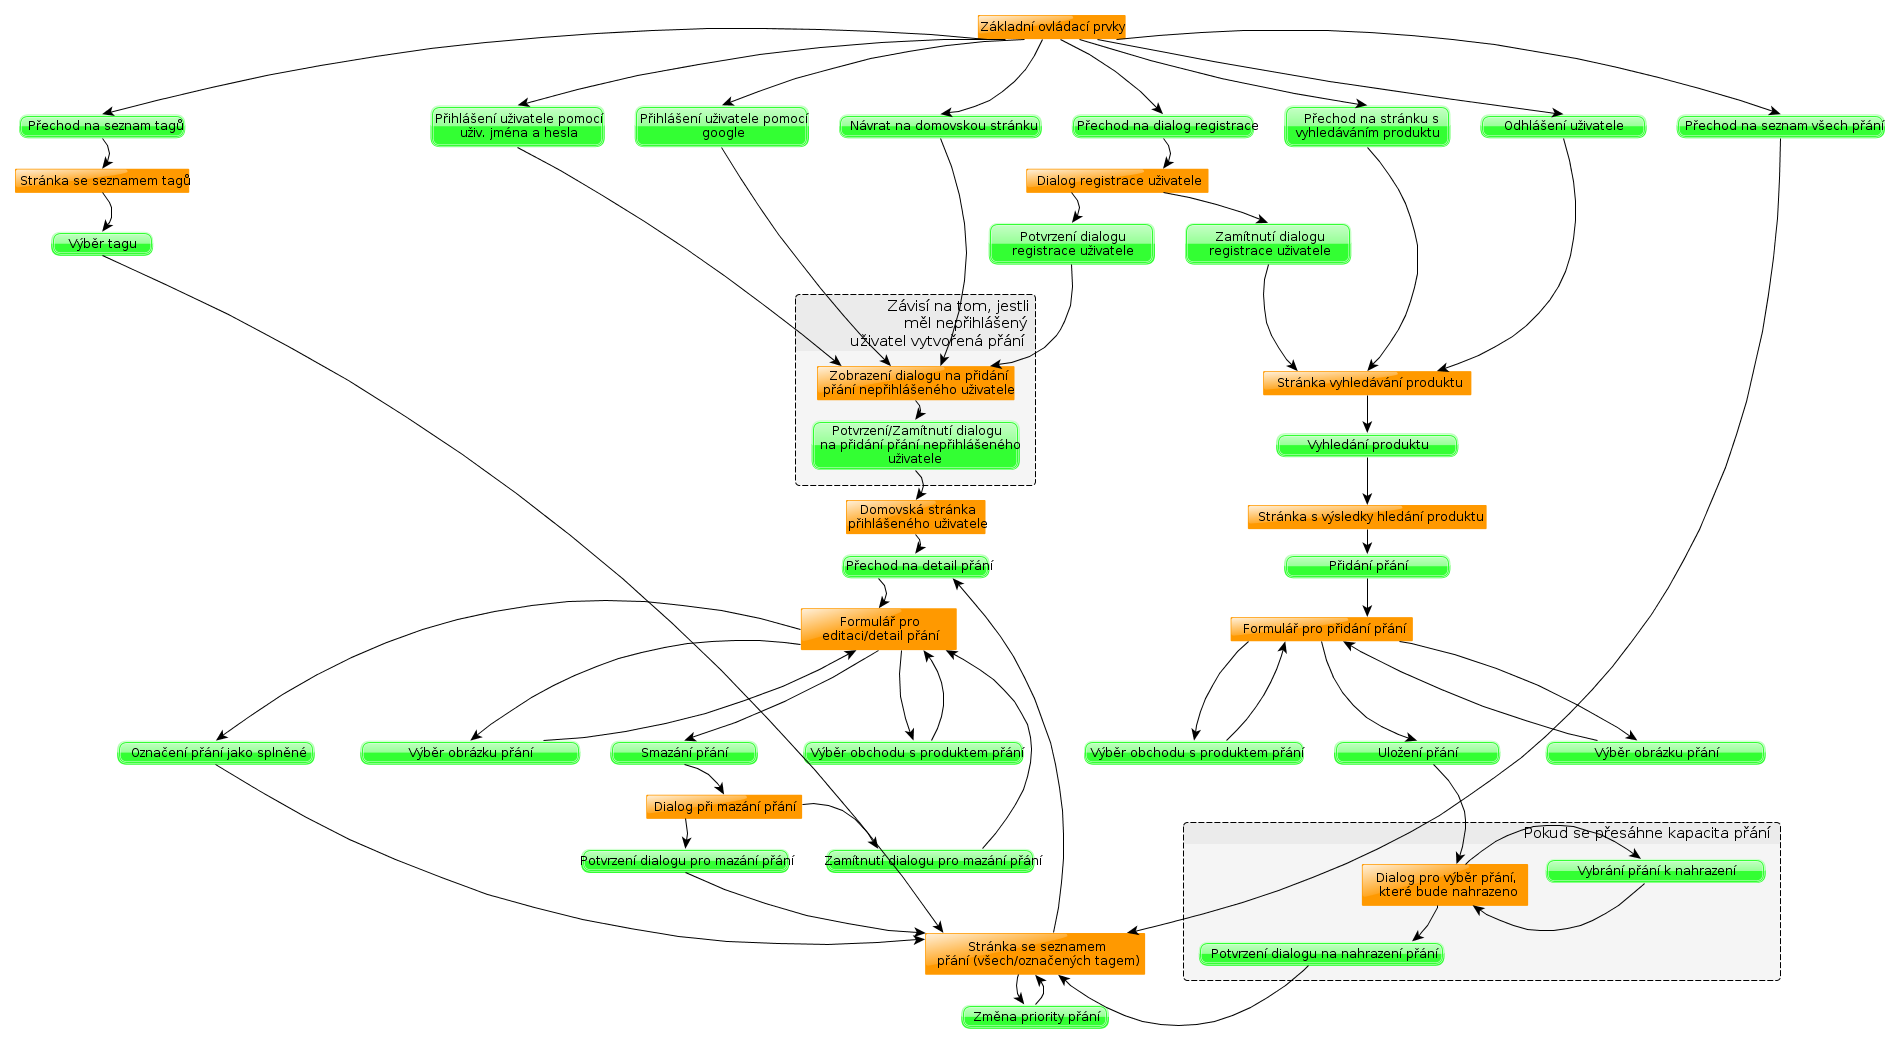
\includegraphics[width=150mm]{./pictures/taskGraph.png}
\caption{Diagram operací pro návrh GUI}
\label{fig:taskGraph}
\end{center}
\end{figure}

\subsection{Wireframe - Drátěný model}
Wireframe je množství ilustrací, které ukazují v malém, nebo velkém detailu obsah každé stránky. Typicky jsou nakresleny pomocí jednoduchých čar, není to vyčerpávající návrh vzhledu. Mimo jiné ukazují jaké informace budou dostupné na jaké stránce. Wireframe je jedním z více kontroverzních dokumentů návrhu uživatelského rozhranní, protože spojují dohromady (tedy nerozlišují mezi) strukturou informací a jejich vizuálním návrhem. Jinými slovy wireframe překračuje hranici mezi strukuturou (jaké mají mezi sebou různé infomrace vztah) a vzheldem (jak budou informace prezentovány na obrazovce)\cite{brown2007communicating}.